\graphicspath{{./images},{./monsters/Blank_Monster/images}}

\DungeonSheetGeometry

\dungeonTitlePage{MarzDarkRed/white}%
	{0cm}%
	{-0.25cm}%
	{height=\paperheight}%
	{Tomb_of_the_Scorpion_King_filter.png}%
	{%
		{TomboftheScorpionKing1}{Page \thepage}{Art}{https://www.imagine.art/}{Tomb of the Scorpion King}{ImagineAI}%
	}%
	{Tomb of the Scorpion King}%
	{black/white}%

\twocolumn[\section*{Dungeon Outlay}
\centerline{\begin{minipage}{\paperwidth}
\begin{tikzpicture}[outer sep=0pt, inner sep=0pt, every shadow/.style={opacity=.8,fill=black}]
	\node {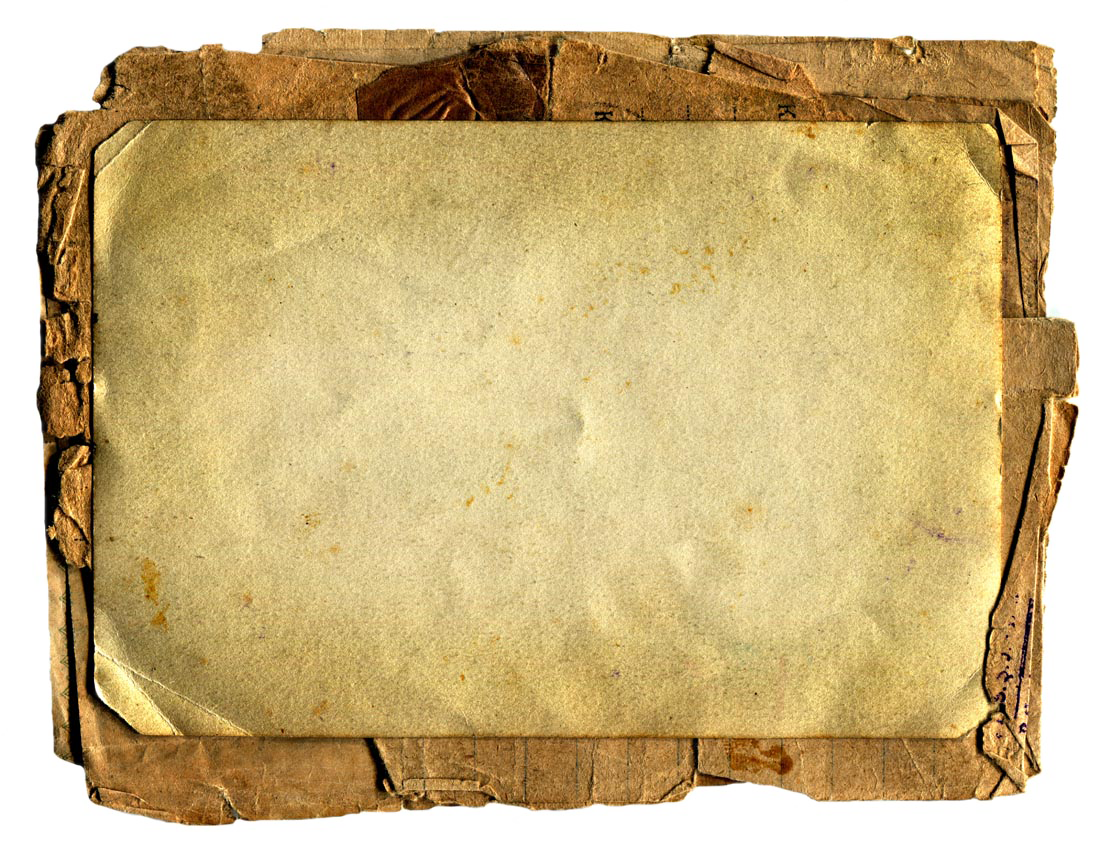
\includegraphics[width=\paperwidth - 8pt, height=14cm]{\PATH regions/stylesheets/images/backgrounds/Dungeons/dungeon_map.png}};
	
	% Guidelines
	\begin{scope}[scale=0.3, every path/.style={black!80, thick}]
		\foreach \y in {0,...,28}
			\draw (-26, -14 + \y) -- ++(52, 0);
		\foreach \x in {0,...,52}
			\draw (-26 + \x, -14) -- ++(0, 28);
	\end{scope}
	
	\begin{scope}[scale=0.3]
		\path[clip, rounded corners=0.5cm] (-1.67\paperwidth + 250pt, -15) rectangle (1.67\paperwidth - 250pt, 15);
		
		\node[inner sep=0pt,outer sep=0pt,clip,rounded corners=0.5cm] {{\transparent{0.7}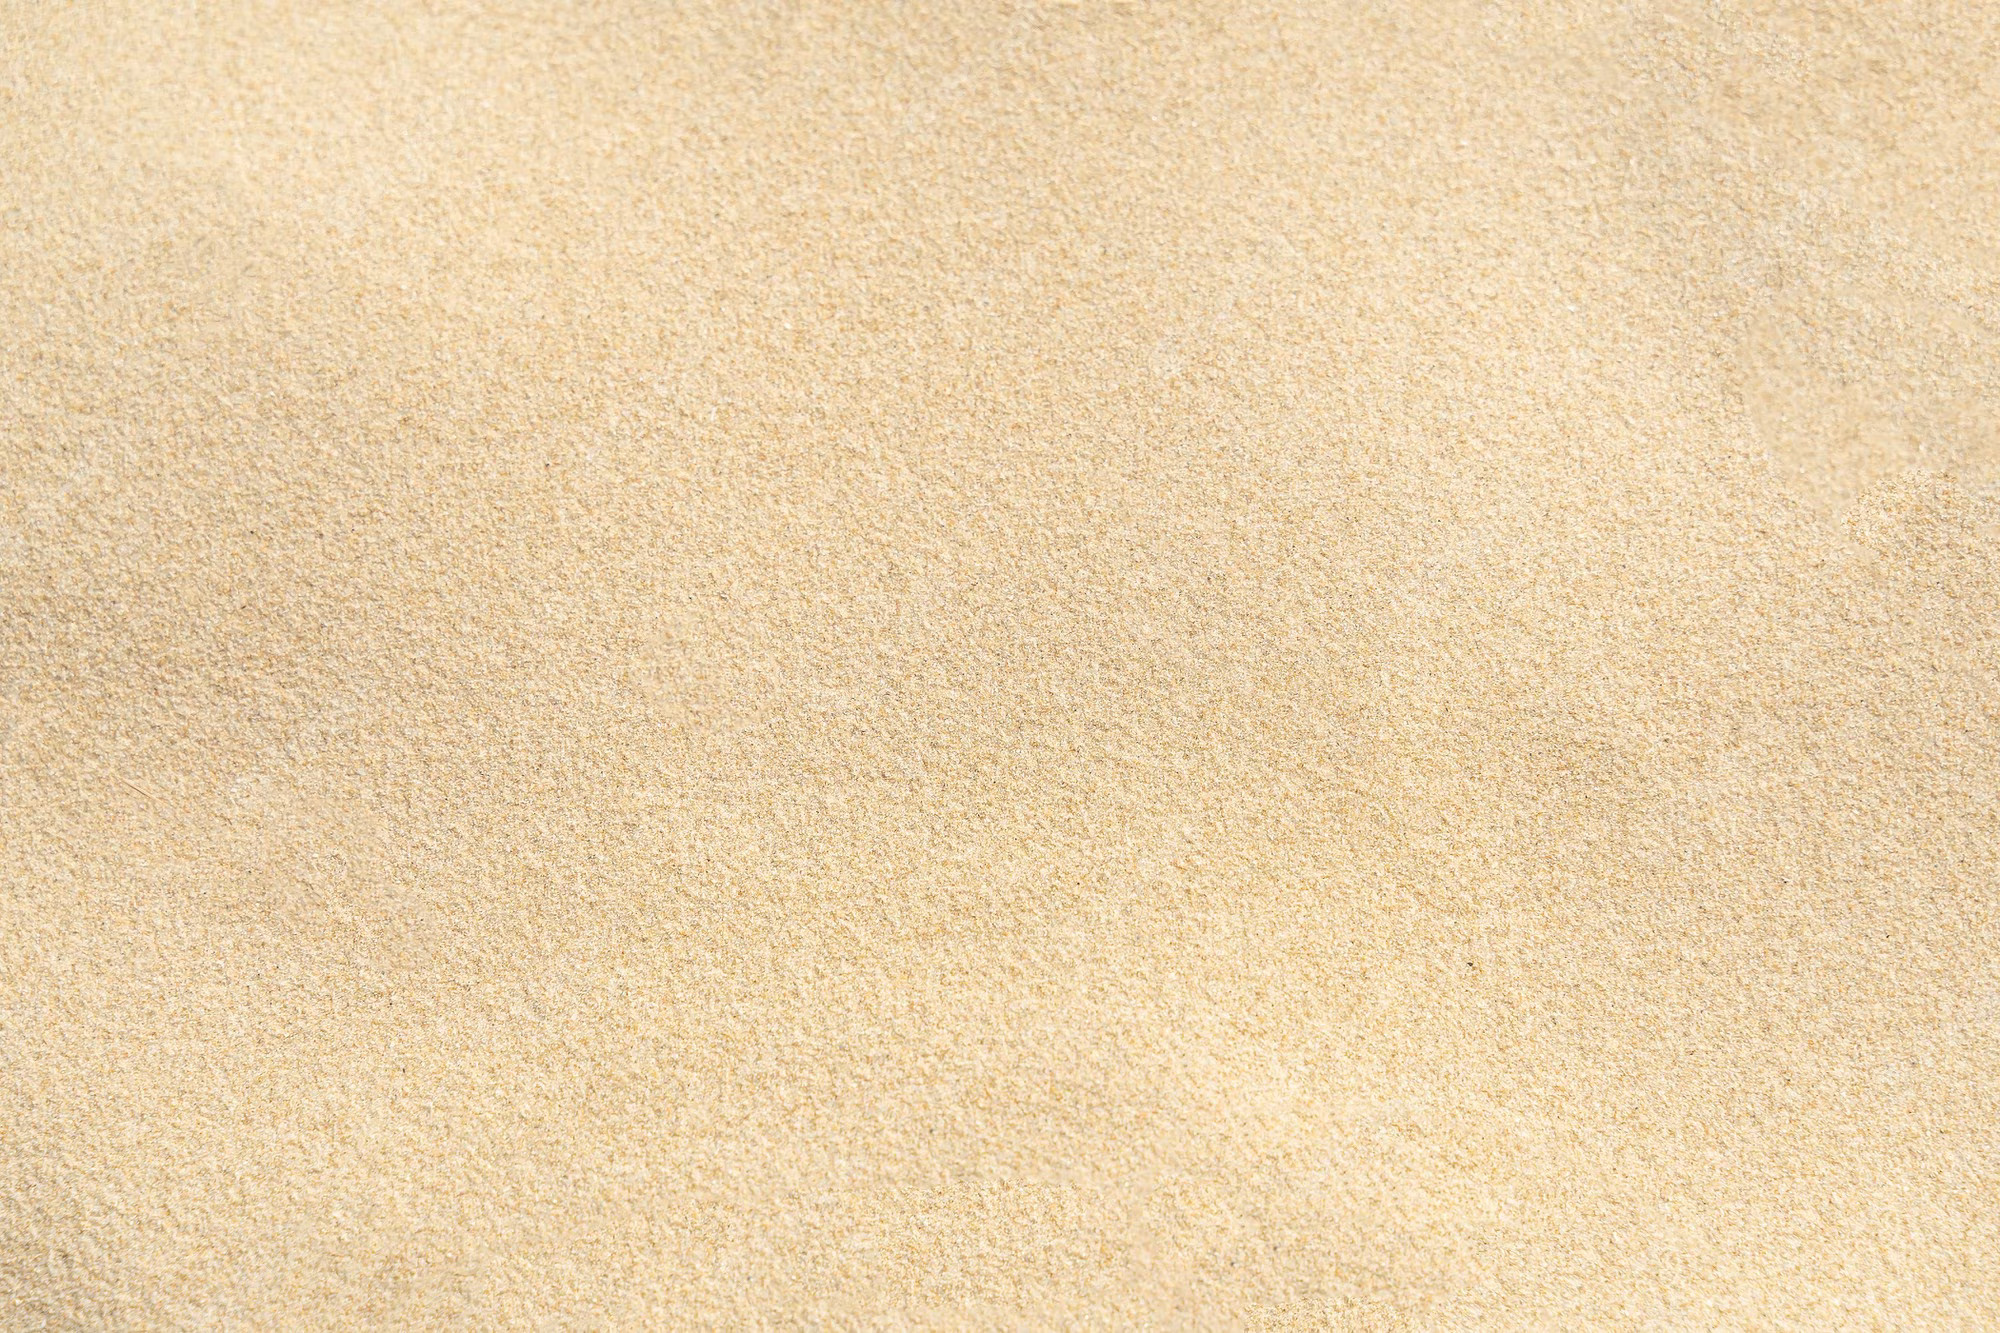
\includegraphics[width=\paperwidth-150pt, height=9cm]{\PATH regions/stylesheets/images/backgrounds/Dungeons/sand_dungeon_texture.jpg}}};
		
		\begin{scope} % Map Features
			% Contour Lines			
			\path[draw] (-4,2) -- ++(0,-5) arc[start angle=-180, end angle=0, radius=3] -- ++(0,5);
			\path[draw] (-4.5,2) -- ++(0,-5) arc[start angle=-180, end angle=0, radius=3.5] -- ++(0,5);
			\path[draw] (-5,3) -- ++(0,-6) arc[start angle=-180, end angle=0, radius=4] -- ++(0,6);
			\path[draw] (-5.5,4) -- ++(0,-7) arc[start angle=-180, end angle=0, radius=4.5] -- ++(0,7);
			\path[draw] (-6,4) -- ++(0,-7) arc[start angle=-180, end angle=0, radius=5] -- ++(0,7);
			\path[draw] (-6.5,4) -- ++(0,-7) arc[start angle=-180, end angle=0, radius=5.5] -- ++(0,7);
			\path[draw] (-7,4) -- ++(0,-7) arc[start angle=-180, end angle=0, radius=6] -- ++(0,7);
			
			% Images
			\node[inner sep=0pt,outer sep=0pt, rotate=180] at (-1,-2.5) {
\includegraphics[height=1.5cm]{Scorpion_Golden_Statue.png}};
			\node[inner sep=0pt,outer sep=0pt, yscale=-1, rotate=-10] at (-6.5,-1.5) {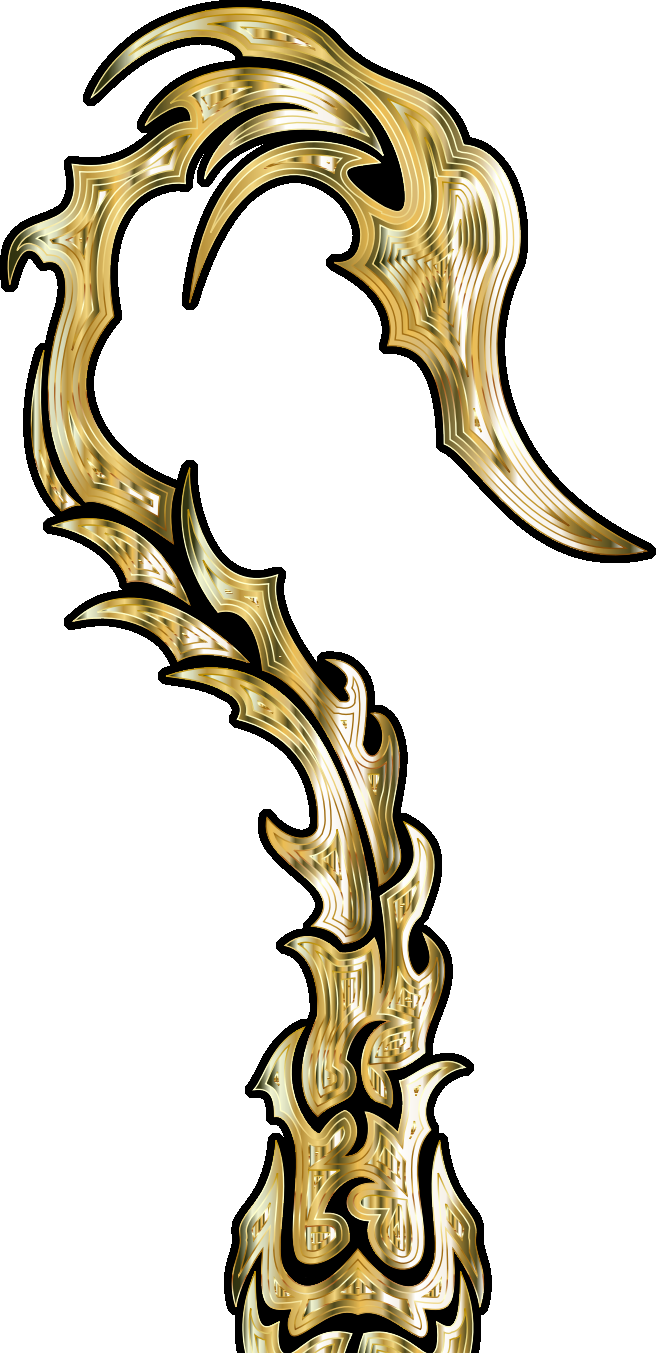
\includegraphics[height=3.6cm]{Scorpion_Golden_Ornament_Tail.png}};
			\node[inner sep=0pt,outer sep=0pt, scale=-1, rotate=-10] at (4.5,-1.5) {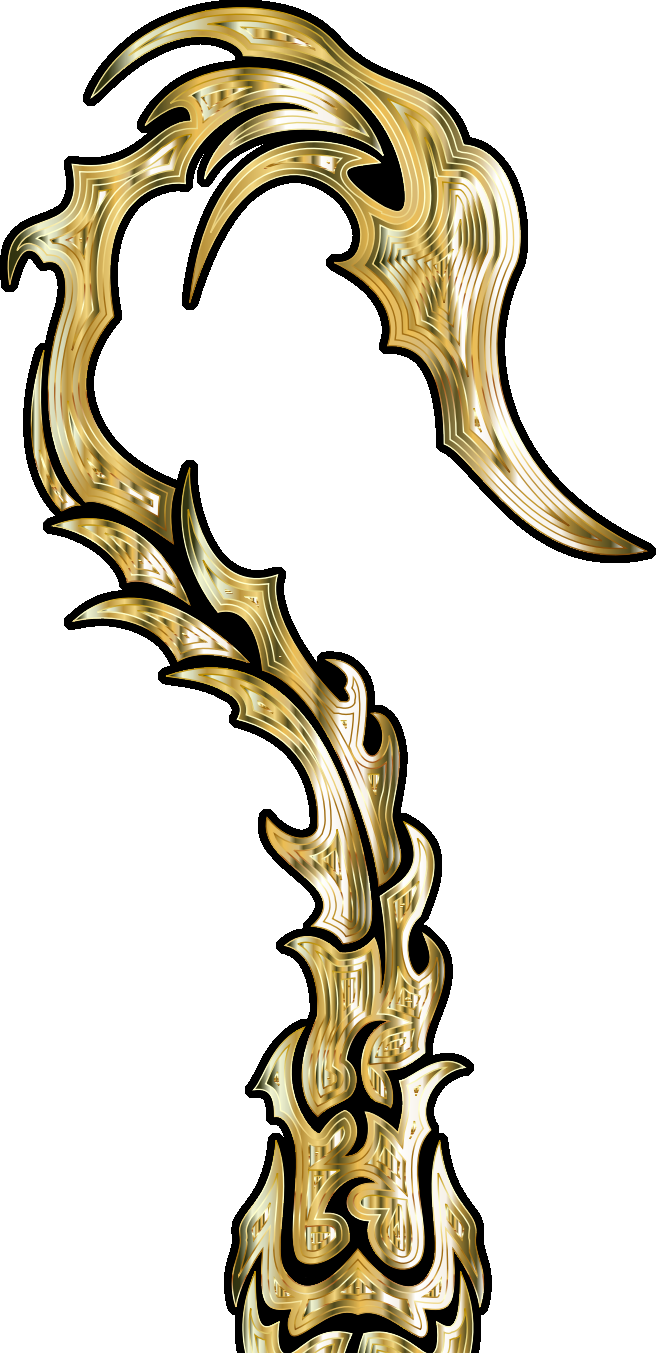
\includegraphics[height=3.6cm]{Scorpion_Golden_Ornament_Tail.png}};
		
			% Traps
			\trapField{8,4}
			\trapField{9,4}
			\trapField{9,5}
			\trapField{8,6}
			\trapField{10,7}
			\trapField{9,8}
			\trapField{10,8}
			\trapField{10,9}
			
			%Stairs
			\stairsField{sand}{13,8}{anchor=south west}{0.3cm}{0.3cm}
			%\stairsField{sandspiral}{-12,9}{rotate=0, yscale=-1}{0.6cm}{0.6cm}
		\end{scope}
		
		\path[clip, drop shadow] (-28,-16)
		-- ++(15,0) -- ++(0,25) arc[start angle=180, end angle=90, radius=1] -- ++(2,0) -- ++(0,-6) arc[start angle=-180, end angle=0, radius=1] arc[start angle=90, end angle=15, radius=4] -- ++(6.275,0) arc[start angle=-195, end angle=-270, radius=4] -- ++(2,0) -- ++(0,7) -- ++(2,0) -- ++(0,-1) -- ++(1,0) -- ++(0,3) -- ++(3,0) -- ++(0,-5) -- ++(-1,0) -- ++(0,4) -- ++(-1,0) -- ++(0,-3) -- ++(-1,0) -- ++(0,-21) -- ++(-24,0) -- ++(0,-5)
		-- (28,-16) -- (28,16) -- (-28,16) -- cycle;
		
		\node[inner sep=0pt,outer sep=0pt,clip,rounded corners=0.5cm] at (0,0) {{\transparent{0.7}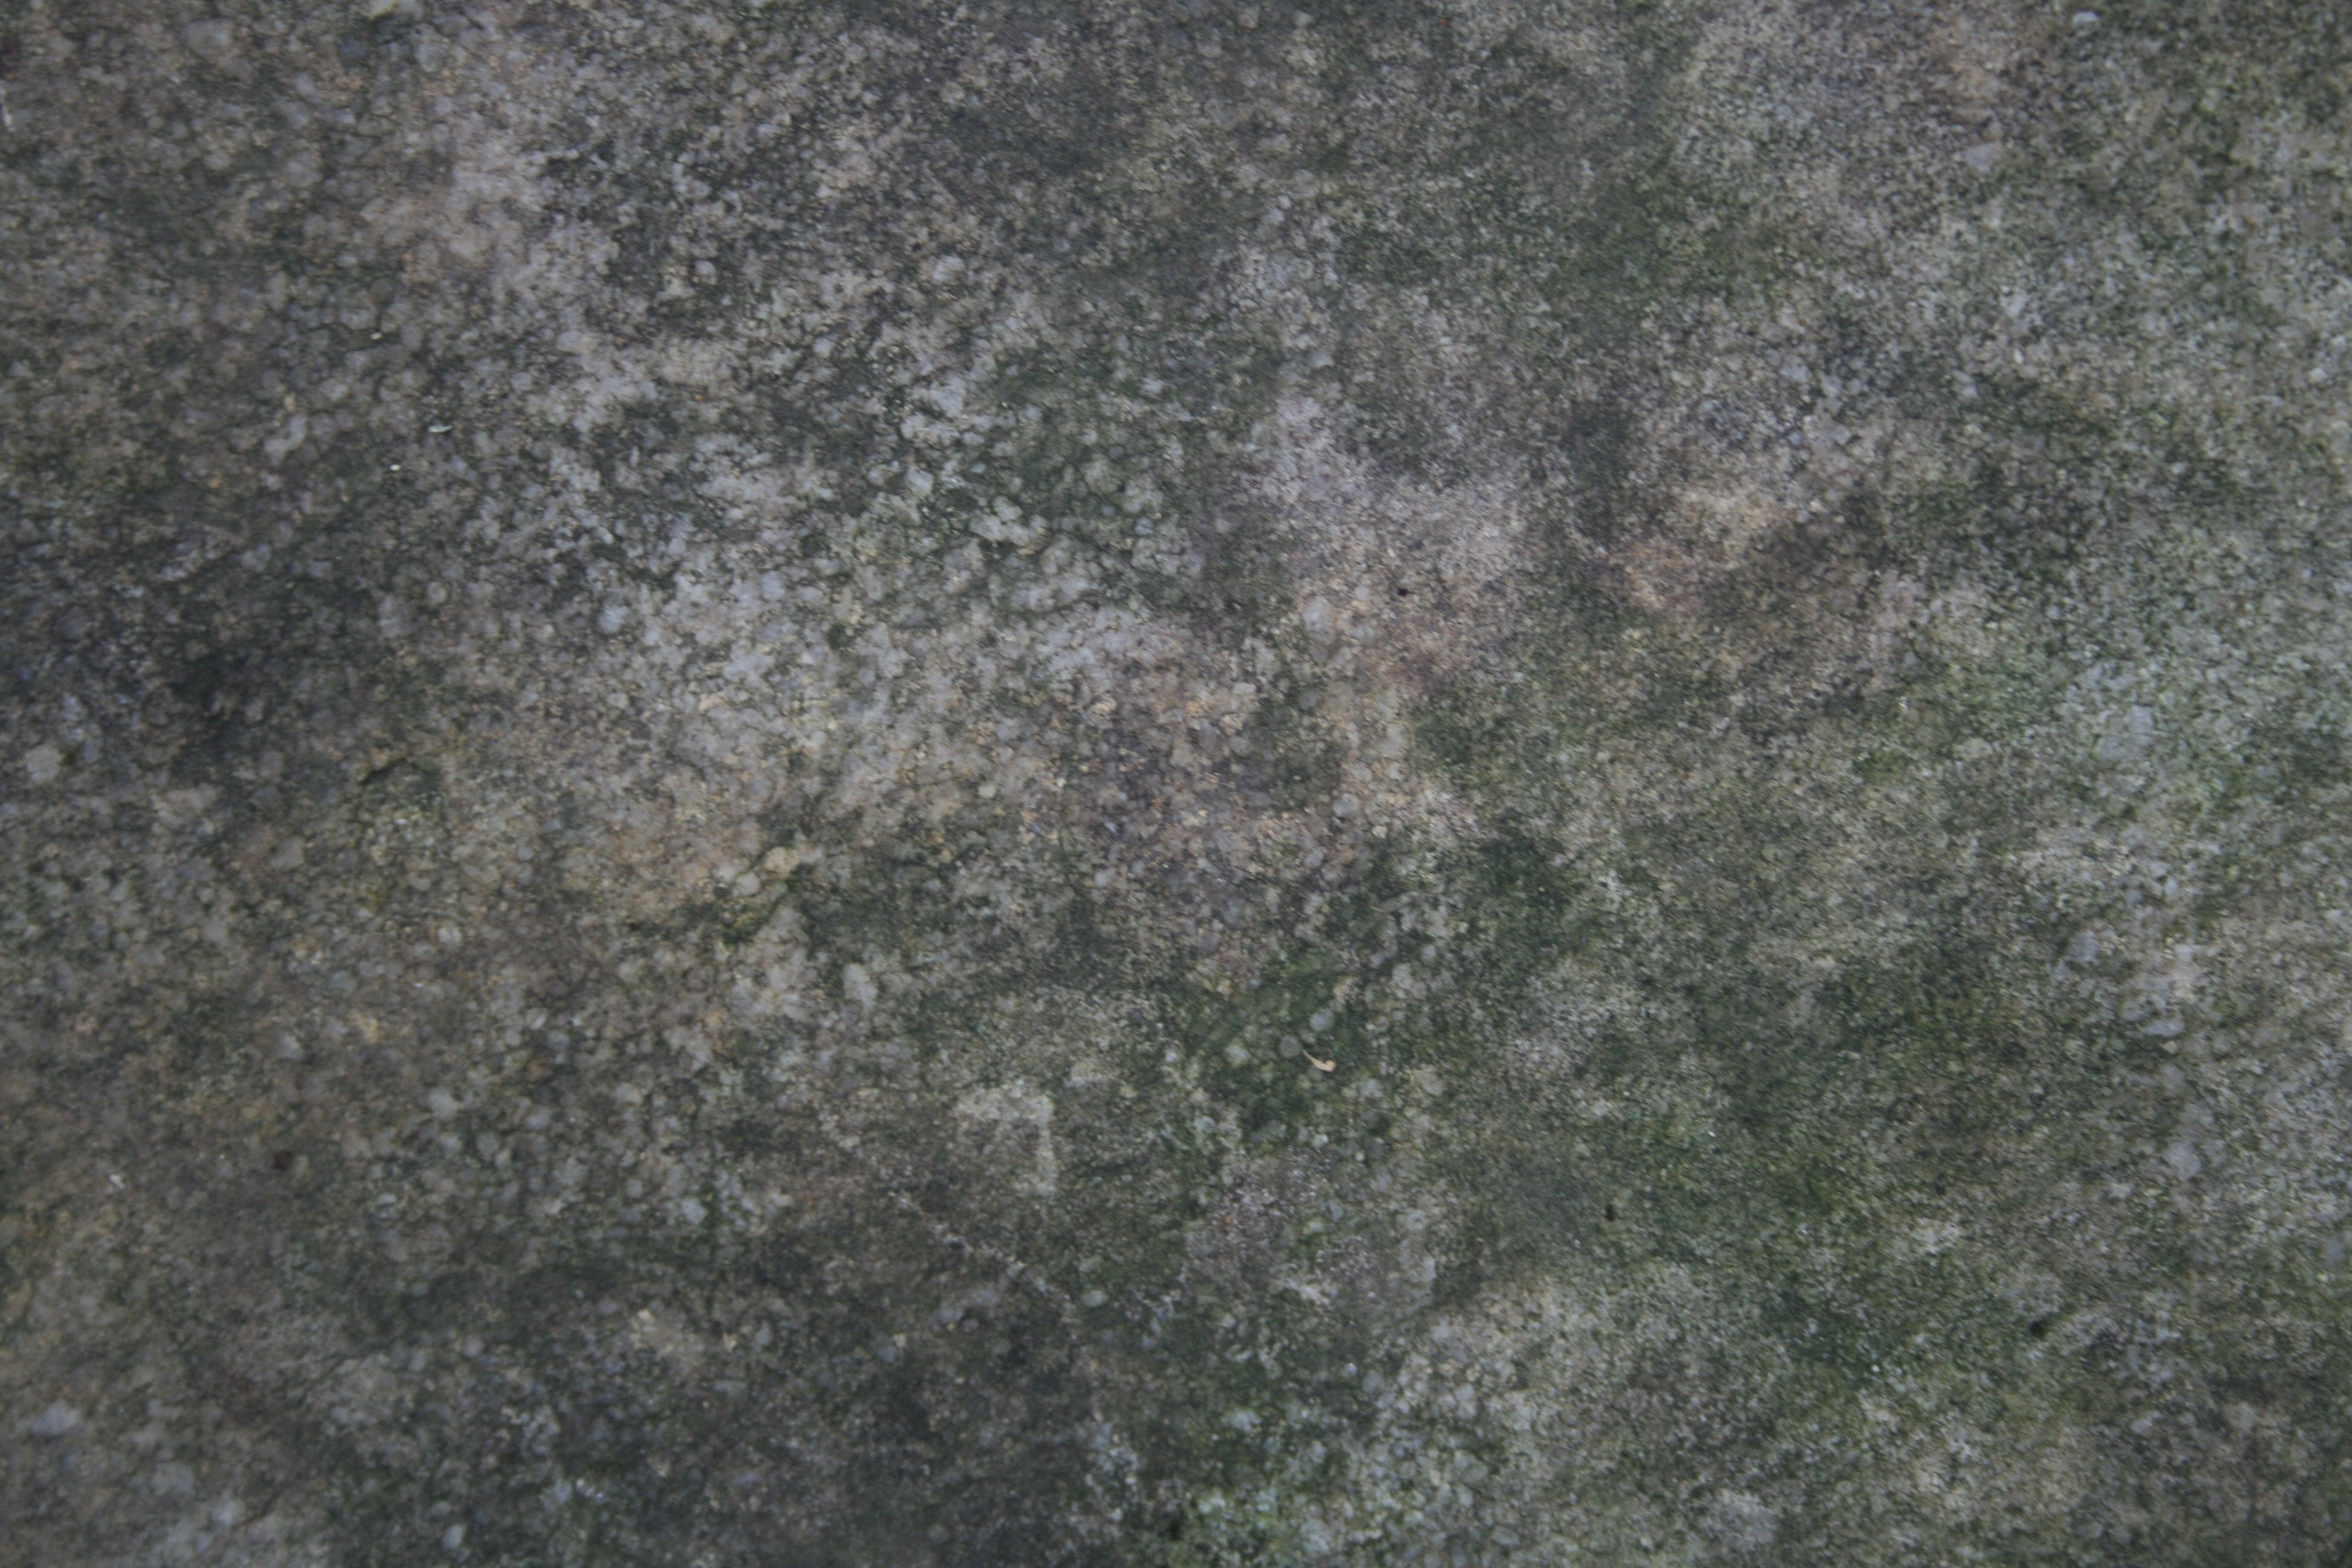
\includegraphics[width=\paperwidth-150pt, height=9cm]{\PATH regions/stylesheets/images/backgrounds/Dungeons/rocky_dungeon_texture.jpg}}};
		
		\path[clip, drop shadow] (-28,-16)
		-- ++(15,0) -- ++(0,5) -- ++(11,12) -- ++(0,2) -- ++(-2,0) -- ++(0,6) -- ++(6,0) -- ++(0,-6) -- ++(-2,0) -- ++(0,-2) -- ++(11,-12) -- ++(0,-5) 
		-- (28,-16) -- (28,16) -- (-28,16) -- cycle;
		
		\node[inner sep=0pt,outer sep=0pt,clip,rounded corners=0.5cm] at (0,0) {\includegraphics[width=\paperwidth-150pt, height=9cm]{\PATH regions/stylesheets/images/backgrounds/Dungeons/sandstone_dungeon_texture.jpg}};		
	\end{scope}
	
	%Doors
	\begin{scope}[scale=0.3]
		%\draw[thick, black] (11,9) -- (11,10) node [pos=.5, right=.02] {\tiny{S}};
		\node[rectangle, thin, draw=black, minimum width=0.1cm, minimum height=0.3cm, inner sep=0, outer sep=0pt, fill=black!50, anchor=west] at (11,9.5) {\tiny{S}};%
		
		\node[inner sep=0pt, outer sep=0pt, anchor=south] at (-1,1) {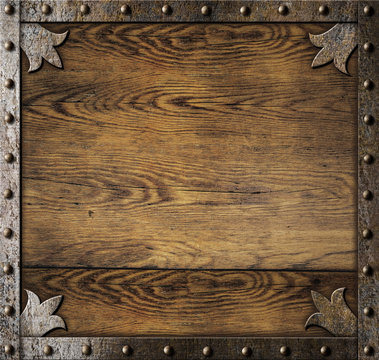
\includegraphics[width=0.6cm, height=0.15cm]{\PATH regions/stylesheets/images/assets/Doors/wooden_door_texture.jpg}};
		
		\stairsField{sandspiral}{-12.04,9}{rotate=0, yscale=-1}{0.6cm}{0.6cm}
	\end{scope}
	
	% Outer Ornaments
	\begin{scope}
		\node[inner sep=0pt,outer sep=0pt, xshift=-0.5\paperwidth+135.5pt] {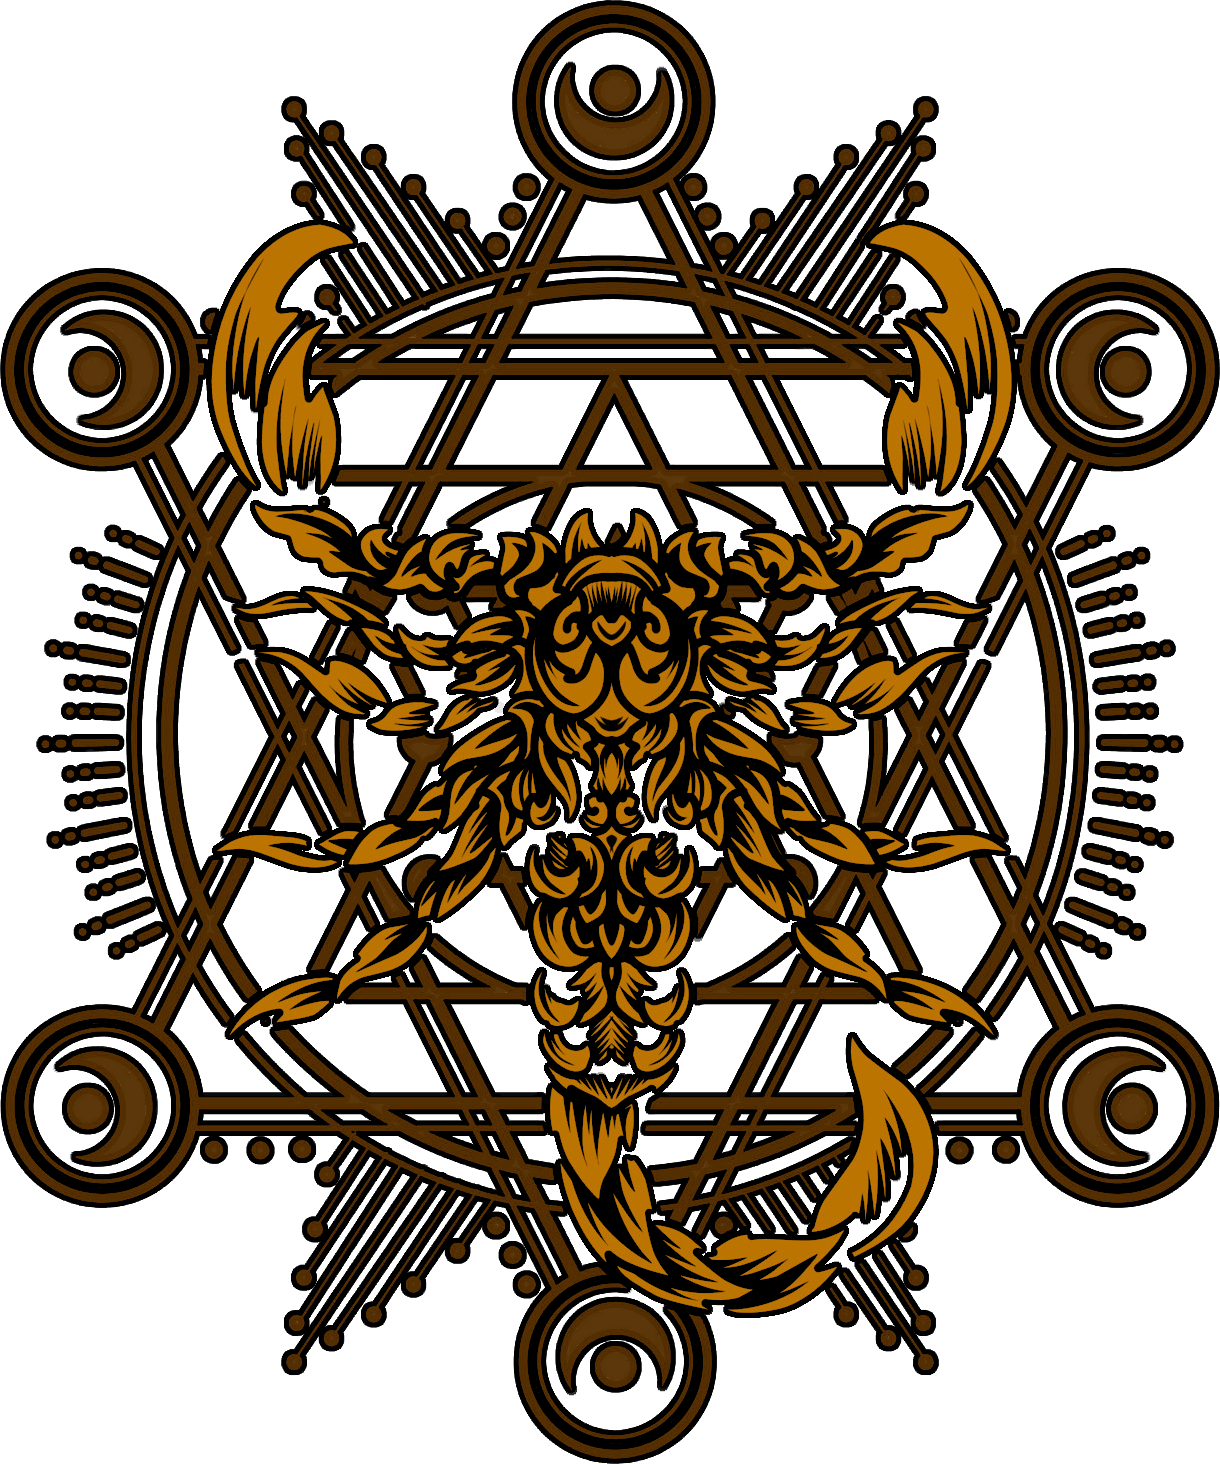
\includegraphics[height=4.5cm]{Scorpion_Ornament_Banner.png}};
		\node[inner sep=0pt,outer sep=0pt, xshift=0.5\paperwidth-145pt, xscale=-1] {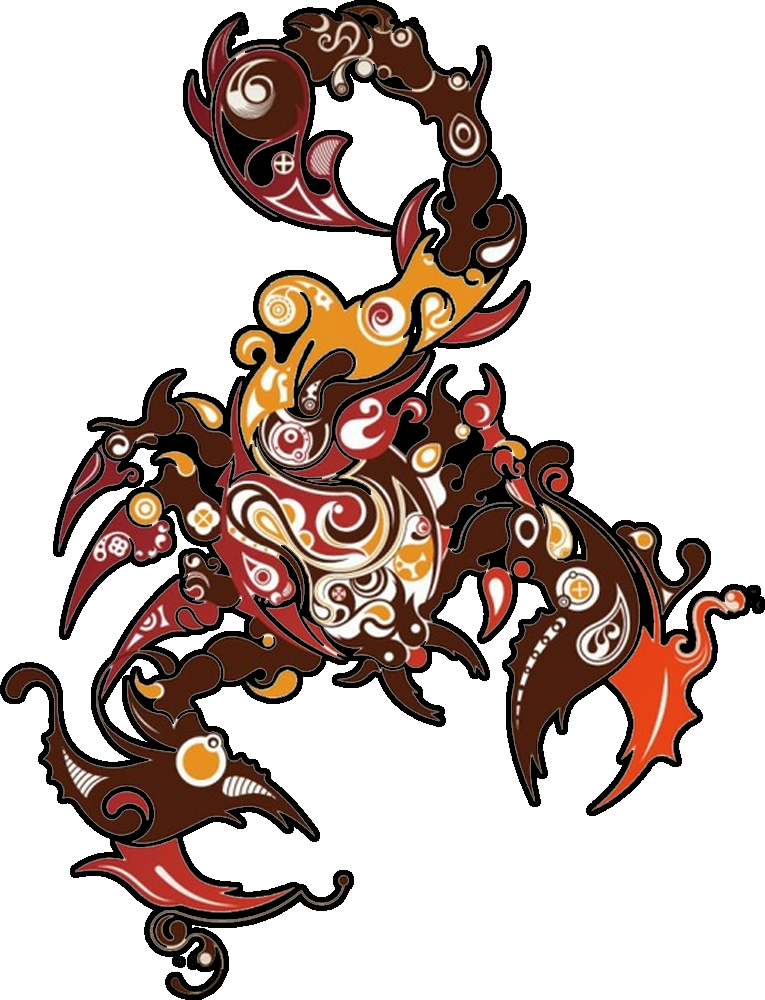
\includegraphics[height=6cm]{Scorpion_Colorful_Ornament.png}};
	\end{scope}
\end{tikzpicture}
\end{minipage}}]

{\entryfont The players come to the end of a large canyon...}